\documentclass[11pt]{rapport_class}
\usepackage[utf8]{inputenc}
% fonts
\usepackage{lmodern}
\usepackage[T1]{fontenc}

% images, pdfs, urls insertion
\usepackage{hyperref}
\usepackage{graphicx}
\usepackage{pdfpages}
\usepackage{parskip}
\usepackage{xurl}

\title{Plan Projet Subjectivity in FakeNews V1}
\author{IAFA-tigable - contributors: Oleiwan Joe, Delmote Adrien..}

\date{13/01/2024}

\begin{document}

\maketitle

\begin{abstract}
Dans le cadre du CLEF 2024, Conferences and Labs of the Evaluation Forum, le laboratoire CheckThat! se concentre sur la Tâche 2, dédiée à l'étude de la subjectivité dans les articles de presse. Notre équipe de Master informatique (IA et Systèmes embarqué) reprend ce projet collaboratif en ciblant l'utilisation de méthodologies basées sur des Modèles de Langage (LLM) et des dictionnaires. Le document fournit un aperçu détaillé du contexte, des techniques et approches de gestion utilisées, soulignant les objectifs du projet ainsi que son organisation.
\end{abstract}

\smallskip
\begin{motsclefs}
\smallskip
\centerline{-Désinformation-}
\centerline{-Subjectivité-}
\centerline{-Détection-}
\centerline{-Subjectivité-}
\centerline{-Objectivité-}
\centerline{-Méthodes-}
\centerline{-Recherche-}
\centerline{-Développement-}
\centerline{-Dictionnaire-}
\centerline{-LLM-}
\end{motsclefs}

\tableofcontents

\chapter{Contexte}
Le laboratoire CheckThat! a été organisé pour la 7e fois dans le cadre de CLEF 2024. Notre but est de réaliser la tâche 2 qui consiste à l’identification de la subjectivité. Dans le but de promouvoir l’intelligence artificielle dans la détection de fragments de texte subjectifs dans les articles de presse. La subjectivité est une caractéristique du langage : en prononçant une énoncé, le locuteur exprime simultanément sa position, son attitude et ses sentiments à l'égard de celle-ci, laissant ainsi sa propre empreinte. Selon le laboratoire, une phrase est considérée comme subjective si elle contient plusieurs critères tels que :
\begin{itemize}
    \item rapporter explicitement l'opinion personnelle de son auteur ;
    \item contenir des expressions sarcastiques ou ironiques ;
    \item contenir des exhortations ou des auspices personnels ;
    \item contenir des expressions discriminatoires ou dévalorisantes ;
    \item contenir des figures de rhétorique explicitement formulées par son auteur pour exprimer son opinion ;
    \item contenir une conclusion tirée par son auteur en dépit d'informations factuelles insuffisantes ;
    \item contenir des intensificateurs qui peuvent être attribués à son auteur pour exprimer son opinion ;
\end{itemize}
La tâche propose des corpus composés de 9 530 phrases annotées manuellement, couvrant six langues - arabe, néerlandais, anglais, allemand, italien et turc.

\chapter{Objectif du projet et parties prenantes}
\section{Objectifs}
Il s'agira de développer des modèles basés sur de l'apprentissage automatique. Les modèles utilisés pourront s’appuyer sur des technologies de type ChatGPT (large language models), LangChain ou/et sur des technologies à base de dictionnaires et de modèles comme les forêts aléatoires.

Les résultats de différents modèles ou différentes configurations de modèles seront présentés
(évaluation de l’efficacité) sur plusieurs jeux de données. Les données fournies sont annotées.

Fonctionnalité minimale : Un modèle apprentissage profond qui marche sur la langue anglaise. Un rapport d’évaluation de la prédiction sera rendu ; plusieurs configurations du modèle seront testés.

Fonctionnalités complémentaires : les différentes langues, différents modèles apprentissage profond ou autre.

\section{Parties prenantes}
\subsection{UE Management}
Présentation de l'UE : Dans le cadre du programme de première année en Master Informatique, l'unité d'enseigement (UE) Mangement de Projet est l'unité qui encadre le projet de 4 mois que nous prenons en charge dans un aspect de gestion de celui-ci. Cette UE fait partie du bloc " professionnalisation " contenant les UE Projet / Initiation à la recherche (TIR) / Stage.

L'évaluation se fera tout au long de l'UE, avec des travaux que l'on doit aux professeurs de management;
Dates et intitulés des Rendus:
\begin{itemize}
    \item Dépôt Rendu kick-off  : 13 janvier 2024
    \item Dépôt Plan projet V1  : 17 février 2024
    \item Dépôt Plan projet V2  : 17 mars 2024
    \item Dépôt Plan project V3 : 14 avril 2024
    \item Dépôt Soutenance finale (Transparent) : avant fin avril 2024
\end{itemize}


\subsection{Client}
Le client est Mme. Josiane Mothe, Porfesseur en Système d'information, Big Data, Recherche d'information, Exploration d'information et Apprentissage automatique à L'institut de Recherche Informatique de Toulouse (IRIT). Responsable et contributrice à plusieurs projets au cours des années, Professeur Mothe nous a proposé ce sujet sur la détéction de la subjectivité pour lutter contre la désinformation du monde actuel.

Nous travaillerons avec Mme Mothe en méthode KanBan en terme de visualisation et adaptation aux objectifs que l'on se fixe au fur et à mesure dans une première phase de recherche, ensuite en méthode Agile en terme de rapidité de travail dans une deuxième phase de développement.
Nous aurons des MileStones à fixer dans un temps future, durant lesquelles nous remettrons à Mme Mothe des rapport intermédiaires sur l'avancement du projet. Cette partie sera détaillé dans la section Organisation de ce document.

\subsection{Capture du besoin}
\begin{center}
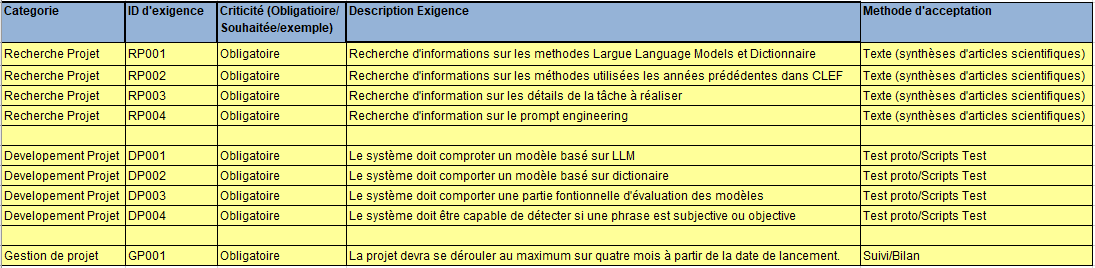
\includegraphics[height=4.2cm]{capture_besoin.png}\\
\tiny
 Source : référentiel projet - Lien : lien github ici ----------------ATTENTION---------------------
\end{center}

\chapter{Organisation}
\section{Organisation globale}
Nous définissons l'organisation globale comme étant le processus et l'ordonnancement des tâches vis à vis d'un cadre d'échange entre l'équipe de projet et la cliente dans le but d'assurer une bonne réalisation du projet sous la période 4 mois entre le 15 janvier 2024 et fin avril 2024.

\subsection{Organisation du travail}
Nous décomposons notre travail en deux phases : 

La première est une phase recherche, dans laquelle nous lisons différents articles scientifiques afin de cerner les anciennes version de ce projet, de voir les méthodes précédemment utilisées et leurs résultats, d'apprendre d'avantage sur la maîtrise des modèles d'apprentissage ciblées, de découvrir de nouveaux aspect liées directement à l'efficience de notre production comme le prompt engineering. 

La seconde est une phase de développement des modèles étudiés durant la phase de recherche. Ces modèles vont analyser les données textuelles et essayer de prédire un jugement sur leur subjectivité. Ensuite, nous développerons le système d’évaluation, qui permet de comparer les résultats des modèles construit avec les résultats de l’équipe de recherche CheckThat!. 

Ces 2 phases ont pour finalité de donnée un avis sur les modèles explorées dans la détection de la subjectivité.

\subsection{Communication}
Afin d'assurer une bonne communication avec la cliente, il a été conclu pendant la réunion de lancement du projet que des réunions de 5 à 15 minutes seront faites en fin de journées sur chacun des deux jours prévus pour le projet dans la semaine, lundi et mardi, dans l'esprit de la méthode Agile. Ces réunions rapides nous permettent de tenir la cliente informé sur une évolution au détail près du projet et de surmonter toute confusion rencontrée sur les tâches définies de manière incrémentale et établir des décisions en temps optimal.

Nous utilisons une communication par mail hors-réunions selon les besoins de gestion qui peuvent subvenir.


\section{Organisation interne de l'équipe}
\subsection{Communication}
Afin de gérer la communication au sein de l'équipe, nous utilisons une plateforme de messagerie instantanée : Discord. Ce logiciel permet de créer plusieurs cannaux textuelles pour différencier entre les tâches discutées, de créer des cannaux vocaux pour se réunir à distance et d'assurer une transmission rapide de documents. Le tout est réalisé sous un même serveur de communication.

\subsection{Suivi des tâches}
Outil de visualtion de tâches Trello : Nous décidons d’utiliser un outil de gestion de projet en ligne inspiré de la méthode KanBan : Trello. Il va nous permettre d’indiquer les différentes tâches à faire, les tâches en cours ainsi que les tâches finies, afin d’avoir un réel suivi sur le projet pour l’ensemble des membres du groupe.

Référenctiel de structure projet : Nous établissons un document excel qui permet de sauvegarder la structuration de projet au niveau OBS (organisation breakdown structure), PBS (project breakdown structure), WBS (work breakdown structure), diagramme de gantt intiale, diagramme de gantt courant.

\subsection{Gestion des ressources et de la production}
Pour gérer nos ressource et nos productions, nous utilisons un système de contôle de version distribué populaire : github. Nous utilisons ce système sous un depôt publique pour organiser les ressources, les logs ainsi que le code produit tout au long du projet. Dans le but, que tout le monde puissent accéder facilement au documents nécessaire ainsi qu’au travail des membres du groupe. GitHub est utilisé pour stocker tout les documents référencé dans le plan projet.

Lien github : \url{https://github.com/fghjklm/Projet_M1_CheckThat-}


\chapter{La Recherche}
\section{Les méthodes précédemment utilisées et les résultats}

\section{Les modèles d'apprentissages automatiques ciblées}
-------------------------TO VERIFY--------------------
Nous regardons différents modèles d’apprentissage automatique à travers des textes scientifiques, dans le but de connaître le modèle en détail ainsi que de pouvoir les implémenter pour notre projet. Notre cliente a commencé à nous parler d’un modèle que l’on peut utiliser. Afin de connaître ce modèle, nous avons lu divers articles scientifiques. Ce modèle est le Large Language Models (LLM), il permet d’interpréter le langage humain. Ils sont basés sur les systèmes de réseau neuronaux artificiels. Les LLMs les plus performants peuvent entretenir une conversation avec des humains (par exemple ChatGPT). 
Les différents rapports de CheckThat de 2023 sur la subjectivité nous ont aussi fait mention de divers modèles comme ...
\section{Le prompt engineering}
Nous regardons les différents prompts dans le but de pouvoir les utiliser avec des LLMs. Les prompts sont des formulations d'instruction aux LLM pour effectuer des tâches. Elle dit aux LLMs comment analyser le texte. Il existe différents types de prompt comme les mother prompts, ce sont des prompts qui permet de faire d’autres prompts. Le but est de recherche et lire des articles scientifiques qui concerne les prompts dans le but de les utiliser au mieux pour avoir de corrects résultats avec les LLMs.





\chapter{Le développement}
\centerline{En construction - Sera établi dans une version future du Plan Projet.}

\chapter{Contrôle Qualité}
\centerline{En construction}


\chapter{État actuel du projet}
POINTEURS

\chapter{Bilan}
\centerline{En construction - Sera établi dans la version 3 du Plan Projet.}
\end{document}
